\Chapter{System Architecture}

\section{Overview}
There are three main server entities in this applicatio, which are Heroku, Facebook, and MongoLab. When the client browser, either from desktop computer or tablet or smart phone, runs the application, it will hit the Heroku server, then the Heroku server will connect to Facebook server to check user authentication. And if the user is not logged-in, the user will be prompted with the Facebook login screen and submit the login data to Facebook server. 

After the user is authenticated to use the application, the application server will connect to MongoLab server to read and write the data. The application server may occasionally go to Facebook server to check the users' friend list or  post to user's wall or check whether the user is still logged-in. 

This application uses HTTPS exclusively for security reasons, except in the local developer environment, where we use unencrypted HTTP,  as shown in Figure ~\ref{fig:deployment}.

\vspace{3em}
\begin{figure}[H]
\begin{center}
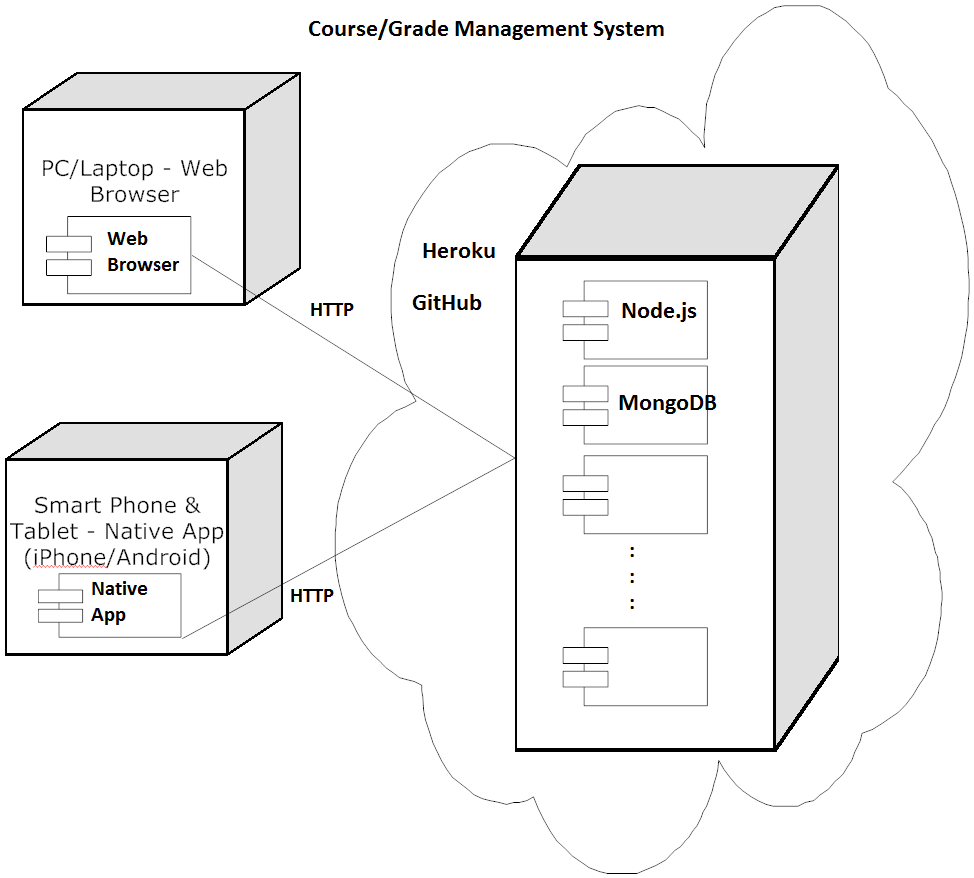
\includegraphics[height=3.8in,width=6.5in]{images/deployment.png}
\caption{Deployment Diagram}
\label{fig:deployment}
\end{center}
\end{figure}


\section{Deployment Workflow}
There are three type of environments used in the deployment workflow: development, staging and production.

Developers work on new features or bug fixes in development branches then only minor updates are committed directly to the stable development branch. Once the features are implemented and/or set of bugs are fixed, they are merged in to staging branch and deployed to staging environment for testing and quality assurance. After testing is completed, the snapshop of staging branch is kept for production deployment, otherwise the process will repeat until the testing is completed. On the release date, the working staging branch is deployed to production environment. 

Figure ~\ref{fig:system-integration} illustrates the deployment workflow.

\vspace{3em}
\begin{figure}[H]
\begin{center}
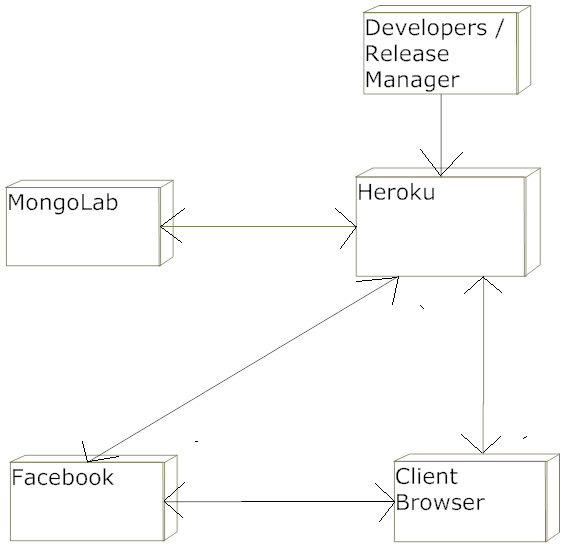
\includegraphics[height=3.8in,width=6.5in]{images/systemIntegration.png}
\caption{System Integration}
\label{fig:system-integration}
\end{center}
\end{figure}


On this project, git is used as code repositories, to manage developments, staging and production branch. And Heroku toolbelt is also used to set the enviroment config variable for each deployment. Heroku allows users to use git to deploy automatically from local repositories. 
 
\subsection{Developers/Release Manager}
In this project, developers first do unit testing in their local machines, then after the system reaches a certain point, the developer himself or assigned release manager will use git to push the changes to staging or production repositories that are connected to respective Heroku servers. 

Below are the commands the developer/release manager uses to start the application in the staging enviroment.
\begin{lstlisting}
$ foreman start
18:43:16 web.1  : started with pid 5540
18:43:16 web.1  : listening on 5000
\end{lstlisting}

Below are the commands for developer/release manager commits changes to master branch of the local repository, then followed by a push to master branch of the remote repository.
\begin{lstlisting}
$ git status
$ git add .
$ git commit -m "message here"
$ git push origin master
\end{lstlisting}

Below are the commands for developer/release manager uses to push to staging environment.
\begin{lstlisting}
$ git push staging master
\end{lstlisting}


\section{Heroku}
In this project there are two sets of heroku instances used: staging and production. 
The application running in Heroku connects to a database server running inside MongoLab using the MongoDB protocol to read and/or write data to database.  Heroku also talks to Facebook servers via Facebook's Open Graph API.

Below is the sample command in Heroku to create staging environment
\begin{lstlisting}
$ heroku create --remote staging
\end{lstlisting}

Below are the sample commands in Heroku to add environmetal variables in remote environment
\begin{lstlisting}
$ heroku config:set S3_KEY=XXX --remote staging
$ heroku config:set S3_SECRET=YYY --remote staging
\end{lstlisting}

\section{MongoLab}
In this project there are three sets of mongo databases used: development, staging and production. It is important to keep the versions of databases since new versions of changes may include changes in database structure, so rolling back or forward the application version would not cause any error. 

Below is the command on how to connect to remote Mongo Database that is hosted in MongoLab

\begin{lstlisting}
$ mongo <servername>.mongolab.com:<portno>/<dbname> 
   -u <dbuser> -p <dbpassword>
\end{lstlisting}

\section{Facebook}
Facebook is playing an important role in this project. Facebook provides user authentication and social media integration. Facebook allows connection using the Facebook API and Open Graph API.

\section{Client Browser}
Client browser uses HTTPS GET for static content, and HTTPS POST for AJAX request to Heroku. And client browser also connects to Facebook server directly using Facebook API and Open Graph API in HTTPS.
 
